\chapter{Experiments}
\label{chap:experiments}

\section{Empirical performance testing}

This section presents the methodology and results of the empirical performance testing of the selected algorithms on the selected benchmarks, using the framework which was designed and implemented for this thesis.
The goal of this phase is to design and run experiments to evaluate the performance of the algorithms on the benchmarks, and based on the empirical results, backup-up by statistical tests, formulate hypotheses on
the relative performance of the algorithms given the problem class, and suggest guidelines for the choice of algorithms and parameters for these algorithms.

\subsection{Methodology}

As it is the case with the literature review, it is important to define a clear and systematic methodology for the empirical performance testing phase. This will ensure the reproducibility of the experiments,
and the validity of the results.

First of all, it is worth noting that the implementation of the different algorithms and benchmarks as parts of a ingle framework, is a key factor in ensuring the fairness of the comparison between the different
algorithms and the validity of the results. Indeed, the different algorithms are implemented in the same language, are queried using a same API, and are run on the same hardware. However, this also means that
errors or small changes in the implementation of the algorithms or benchmarks are possible, and could thus affect the results compared to the original descriptions or implementations.

As one of the goal of the experiments is to evaluate different configurations of the algorithms, the ideal experiment would consist in testing all possible parameters of the algorithms on all possible benchmarks.
However, this is obviously not feasible, as there are infinitely many possible configurations of the algorithms. Therefore, the experiments will be designed to test a subset of the possible configurations, which
will be chosen based on intuition and the literature review. Furthermore, since guidelines for the choice of parameters are sought, experiments will be guided towards
better performance of the algorithms on the problems. This is done by iteratively identifying the parameter values which lead to better performance, and testing more configurations around these values, in order
to refine the choice of parameters.

\subsubsection{Performance measures}

The goal of the experiments is to evaluate the performance of algorithms on benchmark problems, but how is performance defined in this case? The performance of an algorithm can be measured in many way,
depending on the problem and goals. For example, in the case of a sorting algorithm, performance could be measured as the number of comparisons, but in a context where memory usage is important, it is also
worth considering the space complexity of the algorithm.

In the case of this thesis, the following performance measures are considered:

\begin{itemize}
    \item \textbf{Execution time}: the time taken by the algorithm to solve the problem.
    \item \textbf{Quality of the solution}: the quality of the solution found by the algorithm, i.e the fitness of the best performing individual in the final population. For the implemented benchmarks, all
    fitness values are in the range $[0, 1]$, and the higher the fitness, the better the solution.
    \item \textbf{Generations}: the number of generations taken by the algorithm to solve the problem. This metrics only makes sens because of the "early stopping" criterion used in the implementation of the
    algorithms, which stops the algorithm when a fitness threshold is reached.
\end{itemize}

\subsubsection{Testing workflows in practice}

Given the high computational cost induced by the high number of experiments to run, the experiments were run on the high-performance computing cluster (HPC) of DTU.
This will make it possible to benefit from the high number of cores available in the cluster, because of the parallel nature of the implemented testing logic.
More precisely, the central DTU HPC cluster (LSF 10) was used \footnote{\url{https://www.hpc.dtu.dk/?page_id=2520}}.
It contains nodes with 10, 12, 16 or 24 cores. Applications are run on the cluster by mean of job scripts, with the resource manager
parsing the scripts and handling the usage of the available resources. Job scripts contain speciation for the resources requirements, job constraints, a specific queue to use and commands to setup the environment
and run the application. Queues are used to order jobs which are not run immediately.

In addition to running the unit-tests, by having the target set to linux, it also allows to verify that the project should be able to compile on the HPC.
An example of a job script is shown in Listing \ref{lst:job_script}, it runs the $(1 + 1)$ NA algorithm on the \textit{Half} benchmark with a resolution of 100 to 1000, and 1000 runs
for each resolution, and saves the results in CSV files. The configuration of the job script is done using the LSF directives, which are comments starting with \texttt{\#BSUB}.

\begin{lstlisting}[language=bash, caption=Example of a job script, label=lst:job_script]
#!/bin/sh

#### General options
### -- specify queue --
#BSUB -q hpc
### -- set the job Name --
#BSUB -J Bench
### -- ask for number of cores (default: 1) --
#BSUB -n 10
### -- specify that the cores must be on the same host --
#BSUB -R "span[hosts=1]"
### -- specify that we need 4GB of memory per core/slot --
#BSUB -R "rusage[mem=4GB]"
### -- specify that we want the job to get killed if it exceeds 5 GB per core/slot --
#BSUB -M 5GB
### -- set walltime limit: hh:mm --
#BSUB -W 24:00
### -- set the email address --
# please uncomment the following line and put in your e-mail address,
# if you want to receive e-mail notifications on a non-default address
#BSUB -u s222887@dtu.dk
### -- send notification at start --
#BSUB -B
### -- send notification at completion --
#BSUB -N
### -- Specify the output and error file. %J is the job-id --
### -- -o and -e mean append, -oo and -eo mean overwrite --
#BSUB -o ~/Output_%J.out
#BSUB -e ~/Output_%J.err

n_runs=1000

cd ~/code-master

for resolution in $(seq 100 100 1000)
do
      ./target/release/main oneplusonena half -i 500 -n 1 -r $resolution -t $n_runs -o ~/output/oneplusone_na_half_$resolution.csv
done
\end{lstlisting}

\section{Results}

\begin{figure}[h]
    \begin{center}
        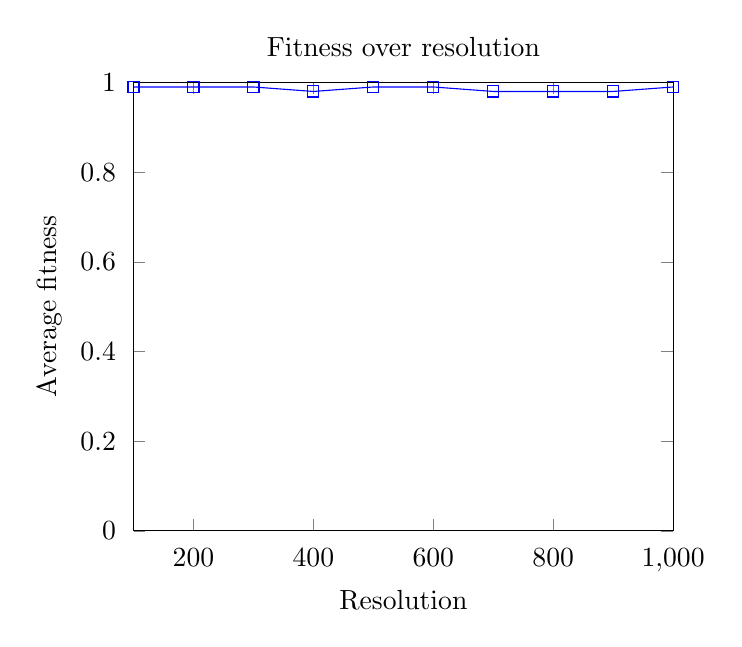
\begin{tikzpicture}
        \begin{axis}[
            % width=12cm,
            % height=7cm,
            title={Fitness over resolution},
            xlabel={Resolution},
            ylabel={Average fitness},
            xmin=100, xmax=1000,
            ymin=0, ymax=1,
            ytick={0,0.2,...,1},
            legend pos=north west,
            xticklabel shift={.1cm},
            yticklabel shift={.1cm} ]
        ]

        \addplot[
            color=blue,
            mark=square,
            ]
            coordinates {
            (100,0.99)(200,0.99)(300,0.99)(400,0.98)(500,0.99)(600,0.99)(700,0.98)(800,0.98)(900,0.98)(1000,0.99)
            };
            % \addlegendentry{Some fancy legend}
        \end{axis}
        \end{tikzpicture}
    \end{center}
    \caption{Some fancy caption}
\end{figure}
